
\documentclass{article}
\usepackage{siunitx}
\usepackage{amssymb}
\usepackage{amsmath}
\usepackage{bm}
\usepackage{subcaption}
\usepackage{cancel}
\usepackage{graphicx}
\usepackage{gensymb}
\usepackage{mdframed}
\graphicspath{{Day5NotesPics/}}
\author{Mann, J}
\title{Day 5 Notes}
\date{September 10, 2015}
\renewcommand{\d}[0]{\mathrm{d}}
\renewcommand{\deg}[0]{\degree}
\newcommand{\note}[1]{\\\\\textbf{\textit{Note: }}#1\\\\}
\newcommand{\matr}[1]{\bm{#1}}
\newcommand{\diag}[1]{\bcancel{#1}}
\newcommand{\dOne}[2]{\frac{\d #1}{\d #2}}
\newcommand{\pOne}[2]{\frac{\partial #1}{\partial #2}}
\newcommand{\dTwo}[3]{\frac{\d^2 #1}{\d #2^2}}
\newcommand{\pTwo}[3]{\frac{\partial^2 #1}{\partial #2^2}}
\newenvironment{aside}{\begin{mdframed}\textbf{\textit{Optional:}}\\}{\end{mdframed}}
\begin{document}
\maketitle{}
\begin{section}{Introduction}
  Last time I introduced the concept of the surface tension as an \underline{excess} pressure. 
  Recall $\matr{P}$ is a rank-2 symmetric tensor so that there is a coordinate transformation $T, TT^{-1} = T^{-1}T = I$ that diagonalizes $\matr{P}$

Assume that the interface is isotropic so that $\diag{\matr{P}} = \begin{pmatrix}
    P_{11} & 0 & 0\\
    0 & P_{11} & 0\\
    0 & 0 & P_{n}
  \end{pmatrix}$

Then \begin{align*}
\gamma = - \int{-\infty}^{\infty} \left(P_{11}(z) - P_n(z)\right) \d z
\end{align*}

In the case of 2D anisotropy
\begin{align*}
  \gamma^{\alpha\beta} = -\int_{-\infty}^{\infty}\left(P_{11}^{\alpha\beta}(z) - P_n(z)\right)\d z
\end{align*}
where $\alpha=1,2$ and $\beta=1,2$
\end{section}
\begin{section}{Developing the Laplace Equation for Interfaces}
	\begin{subsection}{Spheres and Cylinders}
	\begin{figure}[h]
		\centering
			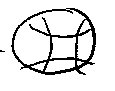
\includegraphics[height=60pt]{sphere}
			\caption{A sphere. In this case $R_1=R_2$}
			\label{fig:Sphere}
	\end{figure}
Let me remind you that 
\begin{align*}
  [P]\equiv \lim\limits_{z\downarrow\Sigma} - \lim\limits_{z\uparrow \Sigma}
\end{align*} 
This is called the jump in the Pressure $P$ across the surface, which is equal to twice the surface tension times the mean curvature. The mean curvature is defined as $2H = \frac{1}{R_1} + \frac{1}{R_2}$, where $R_1$ is the minimum radius of curvature, and $R_2$ is the maximum. The traces of $R_1$ and $R_2$ will always be orthogonal.
  \begin{align*}
    [P]= 2\gamma H; 2H = \frac{1}{R_1} + \frac{1}{R_2}
  \end{align*}
  a sphere, for example, has a constant radius and $R_1 = R_2$. In the example of the soap bubble, there is only one radius, $R$.
  \begin{align*}
		[P]_\text{sphere} = 2\frac{\gamma}{R}
    \label{}
  \end{align*}
	\begin{figure}[h]
		\centering
			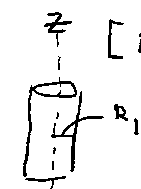
\includegraphics[height=80pt]{cylinder}
			\caption{A cylinder. In this case $R_2 = \infty$}
		\label{fig:Cylinder}
	\end{figure}
Example: Suppose you have a cylinder, has a radius $R_1$, now then I can think of a second radius, that second radius is infinite. Why?

Think of the straight line on the surface, and ask yourself at what distance could I make the radius of a circle conform to the surface of the cylinder? In this case $R_2$ is unboundedly large, thus $2H = \frac{1}{R_1}$, because $\frac{1}{R_2} = 0$.
\end{subsection}

\begin{subsection}{General Case}
	\begin{figure}[h]
		\centering
		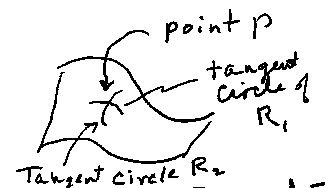
\includegraphics[height=100pt]{tangentCircle}
		\caption{A general surface. $R_1$ is the tangent circle of minimum radius, and $R_2$ is the tangent circle of maximum radius.}
		\label{fig:General Surface}
	\end{figure}
	Imagine that there is a surface that looks like Figure~\ref{fig:General Surface}, and $p$ is the point that you'd like to analyze. Now what is the radius of a circle that will just touch that point? What's the radius in two directions?
	\note{In general:
	\begin{align*}
		H &= \frac{1}{2} \left(\frac{1}{R_1} + \frac{1}{R_2}\right)\\
		K &= \frac{1}{R_1}\frac{1}{R_2}
	\end{align*}
where $H$ is the mean curvature and $\kappa$ is the Gaussian curvature}

	The traces of $R_1$ and $R_2$ are orthogonal. 
\end{subsection}
\end{section}
\begin{section}{Derivation of the Jump $[P] = 2\gamma H$}
	\begin{subsection}
  Recall the work done to vibrate a surface in lecture 4. 
  \begin{align*}
    R  &= \int_{A_0} [P]\zeta(x,y) \sqrt{a}dx dy + \int_{A_0} \gamma\sqrt{a} dx dy\\
    a &= \det{\matr{a}}
  \end{align*}
	Here assume that $[P]$ may depend on $x,y$, but not on $\zeta(x,y), \zeta_1(x,y),$ or $\zeta_2(x,y)$. Also assume the $\gamma$ may depend only on $x,y$. \underline{Geometry} is \underline{next}.
Lets review the metric concept. 
\end{subsection}
\begin{subsection}{The Monge Representation}

	\begin{figure}[h]
		\centering
		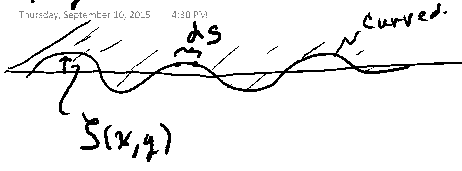
\includegraphics[height=60pt]{vibratingBar}
		\caption{Surface in the act of flapping. A common example of this is an ocean wave.}
		\label{fig:vibrating bar}
	\end{figure}
	\begin{figure}[h]
		\centering
		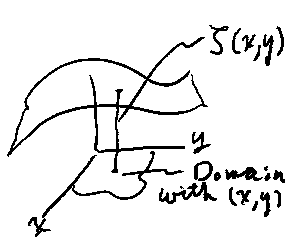
\includegraphics[height=100pt]{zetaSurface}
		\caption{A surface with function $\zeta(x,y)$ in the domain of $(x,y)$}
		\label{fig:zetaSurface}
	\end{figure}
  Define some elevation function $\zeta(x,y)$. In 3-D, $\zeta$ would be the elevation of a plane above the $x$ and $y$ axes. You need to know how to calculate \dots
$$\Sigma =   \begin{cases} x = x\\
  y = y\\
  z = \zeta(x,y)
  \end{cases}$$
  the surface is found at any time in the domain of $x$ and $y$, then calculating $\zeta$
  This is the Monge Representation. Generally, you might define the surface 
  \begin{align*}
    \Sigma  = \begin{cases} x = f(u_1,u_2,t)\\
      y = g(u_1,u_2,t)\\
    z = \zeta(u_1,u_2,t)\end{cases}
  \end{align*}
  The Monge representation is good for almost all cases.
  Example: For a sphere

  \begin{align*}
    \Sigma  = \begin{cases} x = R\cos{\theta}\sin\phi\\
      y = R\sin\theta\sin\phi\\
    z = R\cos\phi\end{cases}
  \end{align*}
  $R$ is the radius, and is a constant. $x_i = x_i(\theta,\phi)$, $i=1,2,3$
  \begin{align*}
    \d E = \begin{pmatrix}
      \dOne{x}{x} & \dOne{x}{y}\\[6pt]
      \dOne{y}{x} & \dOne{y}{y}\\[6pt]
      \dOne{\zeta}{x} & \dOne{\zeta}{y}
  	\end{pmatrix}
      &=\begin{pmatrix}\vec{e}_1 & \vec{e}_2\end{pmatrix}
	= \begin{pmatrix}
      1 & 0\\
      0 & 1\\
      \zeta_1 & \zeta_2
  	\end{pmatrix}\\
    \vec{e}_1 \times \vec{e}_2 &\rightarrow \vec{n};   
	\end{align*}
    $[\vec{e}_1,\vec{e}_2,\vec{n}]$
spans three space.
\begin{figure}[h]
	\centering
	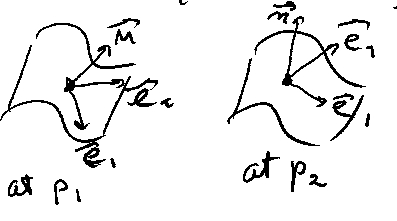
\includegraphics[height=100pt]{p1p2}
	\caption{A demonstration of a general surface. Notice what happens, when you move the point on the surface, the directions change.}
	\label{fig:p1p2}
\end{figure}
  \begin{align*}
    \vec{e}_1 \times \vec{e}_2 &\rightarrow \vec{n}\\
    \frac{\vec{n}}{|\vec{n}|} &= \hat{n}\\ 
    |\vec{n}| &= \sqrt{1  + (\zeta_1)^2 + (\zeta_2)^2}\\
    \d A &= \sqrt{1  + (\zeta_1)^2 + (\zeta_2)^2} \d x \d y 
\end{align*}
 ($\hat{n} = $ unit vector).
  
This is a formula for the differential area. 

    Notice if $\zeta_1 = 0, \zeta_2 = 0,$ then $\d A = \d x\d y$ and the surface is a plane (no curvature.)
\end{subsection}

  \begin{align*}
    R  = \int_{A_0} [P]\zeta(x,y) \sqrt{a}dx dy + \int_{A_0} \gamma\sqrt{a}
  \end{align*}
  $A_0$ is a domain in the $x,y$ plane by choice.
  PICTURE
  \begin{figure}
		\centering
		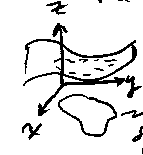
\includegraphics[height=080pt]{aodomain}
  \caption{Example of a domain $A_0$}
\end{figure}
  How to minimize $R$ - Take a derivative, and set the derivative equal to zero.

  Think of minimizing the free energy to find the equilibrium state of the system. You must set a derivative of $R$ to zero as a condition for the minimum.
\end{section}
\begin{section}{The variational Calculus}
  \begin{align*}
    \frac{\partial R}{\partial \zeta} = \text{The variational derivative of R with respect to }\zeta(x,y)\text{, a function}
  \end{align*}
  \note{$R = \int_{A_0} f(x,y,\zeta,\zeta_1,\zeta_2) \d x \d y$ The math \& physics people tell us to compute $\frac{\partial R}{\partial S}$, the result is
	\begin{align*}\frac{\partial R}{\partial \zeta} = \frac{\partial f}{\partial \zeta} - \sum_{\alpha=1}^2 \frac{\partial}{\partial x^\alpha} \frac{\partial f}{\partial \zeta^\alpha} + \dots\end{align*} Do not forget the negative sign.}

	These two terms are all that our functional, $R$, requires. \note{derivatives after $x,y$ are not needed.}
\end{section}
  \begin{section}{Let us take $\zeta$ to be small.}
    By small we mean that $|\zeta|$ is small, $|\zeta_1|$, $|\zeta_2|$ is small. 
    
    Then show that \begin{align*}
      \frac{\partial}{\partial \zeta} \int_{A_0} \zeta\sqrt{a}dx dy &= [P]\\
      \zeta\sqrt{1 + (\zeta_1)^2 + (\zeta_2)^2} &\approx \zeta
  \end{align*}
\begin{aside}
    Take 
		\begin{align*}
		\frac{\partial}{\partial\zeta}\int_{A_0} \gamma \sqrt{a} dx dy = \gamma \int_A \sqrt{a}dx dy
		\end{align*}

    Challenge: Show that 
		\begin{align*}
			\frac{\partial}{\partial\zeta} \int_A \sqrt{a} dx dy = \frac{\partial^2 \zeta}{\partial x^2} ( 1+ (\frac{\partial\zeta}{\partial y})^2) - 2\dOne{\zeta}{x}\dOne{\zeta}{y}\dTwo{\zeta}{x}{y}+ \dTwo{\zeta}{\dots}\dots
		\end{align*}
  \end{aside}

  First consider the surface tension term:
  \begin{align*}
    \pOne{}{\zeta}\int_{A_0}^{}\gamma\sqrt{a}\d x\d y = \gamma\left(\pOne{\sqrt{a}}{\zeta} - \sum_{\alpha=1}^{2} \pOne{}{x^\alpha} \pOne{\sqrt{a}}{\zeta_\alpha}\right)
  \end{align*}
  
	Notice that more generally, $\gamma$ may depend on $x,y$ - but not on $\zeta, \zeta_1,\zeta_2$ for this to work.
	\begin{align*}
		-\gamma \frac{ \pTwo{\zeta}{x}  \left(1 + ( \pOne{\zeta}{y} )^2) - 2 \pOne{\zeta}{x}\pOne{\zeta}{y}\frac{\partial\zeta}{\partial x\partial y} + \pTwo{\zeta}{y} \left( 1+ ( \pOne{\zeta}{x} )^2) }{\left(1 + (\zeta_1)^2 + (\zeta_2)^2\right)^\frac{3}{2}}
	\end{align*}
	
	
	
	
	
	
	The result for small $\zeta$ variations is $2H = \dTwo{\zeta}{x} + \dTwo{\zeta}{y} \therefore$
    \begin{align}
      [P]_\Sigma &= 2\gamma H\\
      [P]_\Sigma &= \gamma(\dTwo{\zeta}{x} + \dTwo{\zeta}{y})
      \label{Eq:Laplace}
    \end{align}
    It takes some geometry to derive the general result: $[P]_\Sigma = \gamma(\frac{1}{R_1} + \frac{1}{R_2})$

		Now we have:

		\begin{align*}
			0 = \int_{A_0}[P](x,y) \zeta\sqrt{a}\d x\d y - 2\gamma H
		\end{align*}

		If I make the assumption that $[P]$ is only a function of $x$ and $y$, and that 
		\begin{align*}
			\zeta\sqrt{a} \approx \zeta(1 + \frac{1}{2}( (\zeta_1)^2 + (\zeta_2)^2))\approx \zeta
		\end{align*}
		is a valid approximation, then we have 
		\begin{align*}
			0 = P - 2\gamma H
		\end{align*}
		Which is the form of the Laplace equation.
  \end{section}
	\begin{section}{Example: Axisymmetric drop shape analysis (ADSA)}
		\begin{figure}[h]
			\centering
			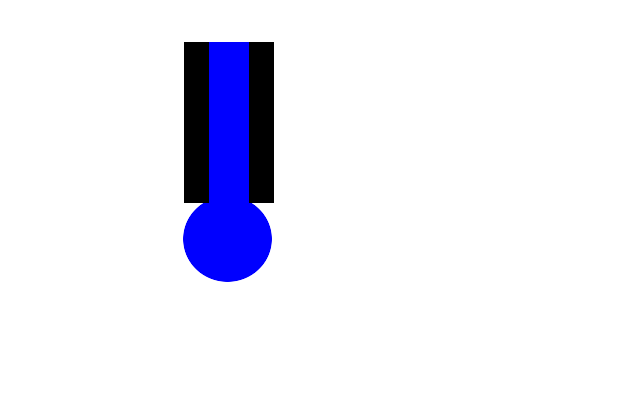
\includegraphics[height=100pt]{ADSA}
			\caption{An example ADSA setup. The black walls are the glass capillary, and the drop has deformed so that it is not quite spherical. }
			\label{fig:ADSA}
		\end{figure}
  The idea is very simple, you have some device (maybe a capillary) and you form a drop. Now take a set of lenses that captures the location of the surface. Then solve Laplace's equation for the best $\zeta(x,y)$ given that you use the pressure jump to compute $\gamma$. One of the reasons for going through this much of the theory, and not more is that the theory really gets rough. The implements used to get the drop-shape analysis have mature implementations. Next time we will go through the various methods of measuring the surface tension, get points of sufficient quality to answer questions that you will deal with if you ever have interfaces 
\end{section}
  \begin{section}{Homework Help}  
    
    \begin{itemize}
      \item $\Pi$ is the ``spreading pressure'', so $\Pi = \gamma_{c=0} - \gamma_c$, so for example, 
	\begin{align}
	  \gamma(T=20 \si{\celsius},C = 0) &= 72\si{\frac{\milli\newton}{\mol}}\\
	  \Pi = 72 - \gamma_c(C=0.007 \frac{\si{mol}}{\si{L}}) &= 72 - 71.2 = .8 \frac{\si{mN}}{\si{m}}
	\end{align}

      \item So if we're looking at the surface tension as a funtion of composition, we're looking at the surface tension of pure solvent, then it goes down. Plot the logarithm\dots

      \item Gamma is the excess. (Where 1 is the solvent) 
	\begin{align*}
	  -\d\gamma &= \bar{s} \d T  - \tau \d P + \Gamma_1 \d\mu_1+ \Gamma_B \d \mu_B. \\
	  \Gamma_1 &= 0, \tau = 0
	\end{align*}
      \item 	Then $-\d \gamma = \bar{S} dT + \Gamma d\mu_B$
      \item Constant $T \rightarrow dT = 0$
      \item $-d\gamma = \Gamma_b d\mu_B$

      \item $\Pi = \gamma_0 - \gamma_c$ (zero - composition)
      \item $\d \Pi = - \d \gamma_c$
      \item $\d \Pi = \Gamma_B \d \mu_B$
      \item You want an inverted version of this equation that you can pop in and play games, make some integrals.

      \item $\Gamma_{max} = $\dots

      \item Using isotherms allows you to get around a problem that you have in getting a numerical derivative. Isotherms allow the problem to be solved without numerical derivatives. Look at the case $\frac{\d \Pi}{\d \mu} = \Gamma$,
      \item so how to best estimate the derivative with the given data? One possibility if you agree with me that the curve looks like this, you might try a polynomial approximation. $y = f(x) + \epsilon(x)$

      \item $d\pi = \bar{S}\d T $
      \item $\bar{S} = (\dOne{\Pi}{T})$
  \end{itemize}



\end{section}
\end{document}
